\chapter{Accessibility Information} \label{sec:chapter-2}

Accessible documents enable readers who use assistive technologies—such as screen readers, braille displays, or text-to-speech tools—to read and navigate content. This supports people with disabilities, including people who are blind, have low vision, or have other print disabilities. Accessible documents also benefit all readers: well-structured documents are easier to navigate, reflow better on small screens, and can be more reliably parsed by search engines and automated tools.

While this template provides auto-tagging support, it does not make a document fully accessible by itself. Authors still need to use semantic \LaTeX{} commands and provide the information that cannot be inferred automatically, such as alt text for figures and table headers. The following sections include guidance on making content accessible.

\section{Headings}

Use \LaTeX{} sectioning commands to create headings, so that they can be automatically tagged with the correct heading levels in the PDF and displayed by PDF viewers as a document outline.

\begin{itemize}
    \item \verb|\thesistitle| creates the top level tag Title
    \item \verb|\chapter| creates a level 1 heading (H1)
    \item \verb|\section| creates a H2
    \item \verb|\subsection| creates a H3
    \item \verb|\subsubsection| creates a H4
    \item \verb|\paragraph| creates a H5
    \item \verb|\subparagraph| creates a H6
\end{itemize}

Make sure to use heading levels in order and avoid skipping heading levels.

\section{Figures}

NOTE: Figure captions go below figures and must use the “Caption” style in order to auto-populate a List of Figures. 

NOTE: All images must include alt-text. 
%To insert alt-text to images, hover over the image > right click > view alt text > input the description for the image



\begin{figure}[ht]
    \centering
    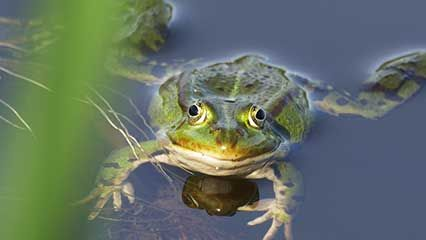
\includegraphics[alt={a green frog is laying in a pond}, width=0.7\linewidth]{figures/frog.jpg}
    \caption{A frog on a log}
    \label{fig:frog}
\end{figure}

\TeX{} Live 2025 or newer versions have auto tagging for figures. However, alt text still needs to be added manually in the \LaTeX{} source; it is not automatically generated when a figure is created. 

To insert alt text, add the “\verb|alt|” key inside the \verb|\includegraphics| command, as in \texttt{alt=\{a green frog is lying in a pond\}}. See the \LaTeX{} code example in \autoref{fig:frog}. This alt text will then be automatically included in the PDF tags.

In general, useful alt text should begin with a high-level summary of the figure, followed by as much relevant detail as possible to help readers understand the figure’s meaning or purpose. For more detailed guidance, see SIGACCESS’s guide \cite{trewin2019} on describing figures.


\begin{figure}[ht]
    \centering
    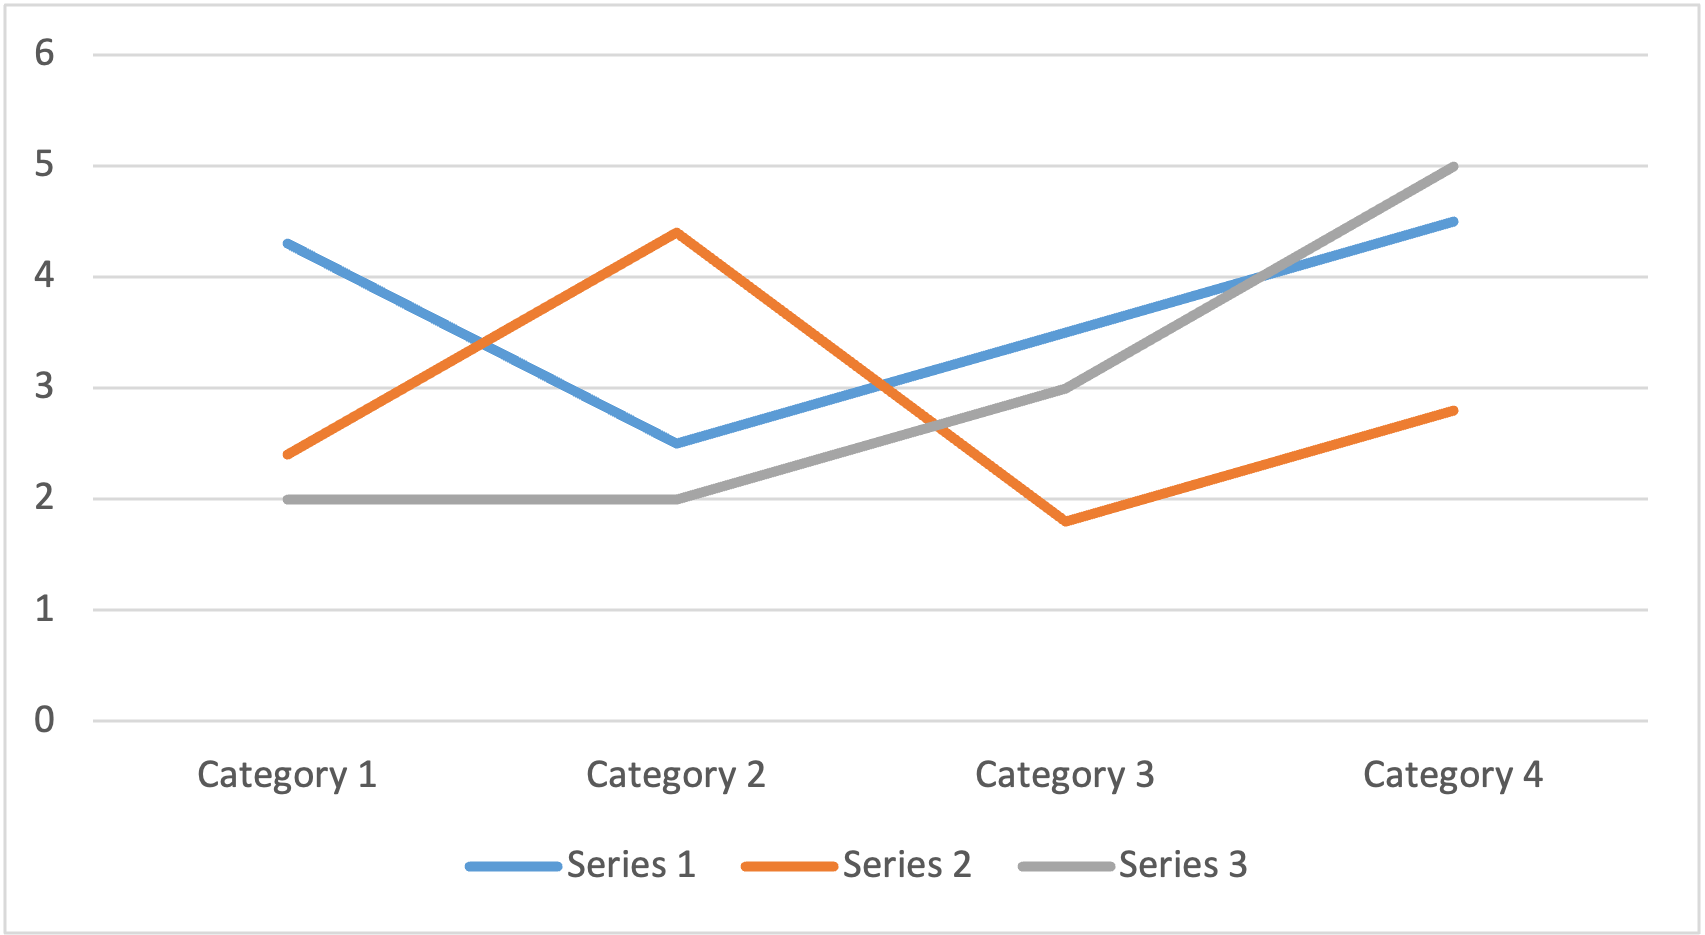
\includegraphics[alt={Line chart comparing values for 3 series across 4 categories. x-axis shows Categories 1 through 4, y-axis ranges from 0 to 6. Overall, Series 1 and Series 3 end higher than they begin, while Series 2 rises and falls. Series 1 decreases at first, then increases. Series 2 peaks in Category 2 and reaches its lowest value in Category 3. Series 3 stays flat at first, then increases. Approximate values from Categories 1 to 4 are: 4.3, 2.5, 3.4, 4.5 for Series 1; 2.4, 4.4, 1.8, and 2.8 for Series 2; 2.0, 2.0, 3.0, and 5.0 for Series 3.}, width=0.7\linewidth]{figures/chart_template.png}
    \caption{Example chart}
    \label{fig:chart}
\end{figure}



\autoref{fig:sourcecode} is just for illustration purposes, as is \autoref{tab:coordinates}. Note that these figures and tables are made of text and are highlightable. No images of text. 


\begin{figure}[ht]
\begin{verbatim}
#include <iostream>
int main(int argc, char** argv) {
  std::cout << "Hello World." << std::endl;
  return 0;
}
\end{verbatim}
  \caption{Example source code.}
  \label{fig:sourcecode}
\end{figure}






\section{Tables}


%NOTE: Table captions go above tables and must use the “Caption” style in order to auto-populate a List of Tables. % from the Word template
NOTE: Table captions go above tables and auto-populate a List of Tables. 
If any caption is more than four lines, all captions must be single spaced. In general, we recommend single spacing captions. 

Tables should be created as real \LaTeX{} tables using the \verb|tabular|, \verb|tabularx|, or similar table environments, rather than inserted as images of tables.

Each table should have its header row defined. Typically, the header is the first row. To mark the first row as the header row, add \verb|\tagpdfsetup{table/header-rows={1}}| above the table environment (before \verb|\begin{table}|). See the \LaTeX{} code example in \autoref{tab:coordinates}.
If the table has multiple header rows, list all header row numbers. For example, if rows 1 and 2 are both header rows, use \verb|\tagpdfsetup{table/header-rows={1,2}}|.


\tagpdfsetup{table/header-rows={1}}
\begin{table}[h]
  \centering
  \caption{Example coordinates.}
  \begin{tabular}{|rr|r|}
    \hline
    $x$ & $y$ & $z$ \\
    \hline
    14 & 12 & -2 \\
    0 & 33 & -25 \\
    -3 & 11 & 22 \\
    4 & 4 & 6 \\
    \hline
  \end{tabular}
  \label{tab:coordinates}
\end{table}


\tagpdfsetup{table/header-rows={1}}
\begin{table}[htbp]
\centering
\caption{City or Town Distance Matrix}
\label{tab:city_distance}
\begin{tabularx}{\textwidth}{|>{\raggedright\arraybackslash}p{3cm}|*{5}{>{\raggedright\arraybackslash}X|}}
\hline
\textbf{City or Town} & \textbf{Point A} & \textbf{Point B} & \textbf{Point C} & \textbf{Point D} & \textbf{Point E} \\ \hline
Point A & --- &     &     &     &     \\ \hline
Point B & 87  & --- &     &     &     \\ \hline
Point C & 64  & 56  & --- &     &     \\ \hline
Point D & 37  & 32  & 91  & --- &     \\ \hline
Point E & 93  & 35  & 54  & 43  & --- \\ \hline
\end{tabularx}
\end{table}



\section{Math Equations}

\TeX{} Live 2025 can auto tag math equations as “Formula” and attaches the corresponding MathML to the PDF. Compatible PDF viewers, such as Adobe Acrobat Pro, can use this MathML to make equations available to assistive technologies. The generated MathML can be found in the PDF’s attachments panel using Acrobat Pro.

$$ \int_1^{12} \frac{x^2}{5 - \sqrt{5}} \,dx $$

We can also try labeling equations.
\begin{equation}\label{eqn:einstein}
E=mc^2
\end{equation}
Then we can refer to \autoref{eqn:einstein}.

